%!TEX root = TFG.tex

\lstset{frame=single,basicstyle=\ttfamily\small}

\chapter{Análisis de objetivos y metodología}

En esta sección definiremos los objetivos del trabajo y se realizará un análisis sobre las decisiones tomadas.

\section{Objetivos}

El objetivo de este trabajo será entrenar un modelo de machine learning que sea capaz de identificar cada dispositivo respecto de los otros que se encuentran bajo análisis. Para realizar esto mediremos la desviación de los respectivos relojes (\textit{clock skew}).

Esta desviación se ver como la diferencia entre un reloj teóricamente exacto $c_{ex}$ y el reloj del dispositivo a analizar $c$ en un tiempo $t$. Con esto definimos la desviación del reloj $c$ en el tiempo $t$ como:
\begin{gather*}
    offset(c(t)) = c(t) - c_{ex}(t)
\end{gather*}
Una vez tengamos esta desviación de reloj para cada uno de los dispositivos, estudiaremos como varía esta desviación a lo largo del tiempo. Para esta labor definimos:
\begin{gather*}
    \Delta offset\left(c\left(t\right)\right) = offset\left(c\left(t\right)\right) - offset\left(c\left(t - 1\right)\right)
\end{gather*}

Una vez tenemos los datos recogidos, estudiaremos distintos valores estadísticos que, presumiblemente, nos aportarán información para distinguir los distintos dispositivos.

Por último analizaremos un conjunto de algoritmos de Machine Learning entrenados con un subconjunto estos datos, para evaluar su capacidad de identificar los dispositivos.

\section{Algoritmos de Machine Learning}

El Machine Learning se trata al fin y al cabo de una búsqueda, una búsqueda de formas alternativas de hacer algo. Para ello se busca en estructuras muy similares a las previas. Para modificar una estructura y seguir con la búsqueda nos valemos de sucesos que hayan acontecido, entonces, evaluamos si han mejorado y nos quedaremos como estructura para la siguiente iteración con la que más mejore a la previa. Para realizar estas operaciones necesitamos una forma de cambiar de estructura y una forma de evaluar si hemos mejorado.

Con esta forma de trabajar vemos que el programa no tiene que resolver la tarea sino autoajustarse para obtener mejores evaluaciones cada vez. El programador por tanto no pone el programa sino proporcionar al programa la mejor estructura modificable y a continuación alimentar al sistema con datos. Aportamos por tanto ejemplos o premios que ayudan al programa a autoajustarse. Existen tres tipos de aprendizaje: 

\begin{itemize}
    \item \textbf{Supervisado}: al sistema se le proporcionan ejemplos de cuales la solución es conocida. Una variante sería el semi-supervisado en el que sólo una parte de los datos tienen solución conocida.
    \item \textbf{No Supervisado}: al sistema se le proporcionan datos que no tienen una solución conocida, esperando que el sistema nos proporcione conocimiento que intuimos que existe en dichos datos. Un ejemplo sería el \textit{clustering} que agrupa los datos por similitudes.
    \item \textbf{Por refuerzo}: al sistema no se le pasan ejemplos de datos, sino que se le premia o castiga por distintas conductas que desarrolla automáticamente. Al final el sistema, que busca obtener más premios, se comportará de la forma que queremos.
\end{itemize}

\subsection{Tratamiento de los datos}

Para obtener un resultado de cuan bueno es un modelo (algoritmo) que queremos usar debemos dividir el conjunto de datos inicial en dos conjuntos: \textbf{datos de entrenamiento} y \textbf{datos de test}. Con los datos de entrenamiento el algoritmo se ajusta y aprende de los datos, y con los datos de test comprobamos los resultados que obtenemos del algoritmo ante datos que no ha visto antes.

Para realizar una comparación entre distintos modelos y queremos ver cuál es el que mejor se ajusta a nuestros datos debemos dividir el conjunto de datos de entrenamiento en otros dos conjuntos: \textbf{conjunto de entrenamiento} y \textbf{conjunto de validación}. Con este último podemos evaluar la capacidad de generalizar de nuestro algoritmo.

Con esta segunda división obtenemos el algoritmo que mejor se adapta a nuestros datos, pero no un modelo final. Para tener un modelo final lo entrenaremos con el conjunto de datos de entrenamiento en su totalidad y lo evaluaremos con los datos de test.

\subsection{Algoritmos de aprendizaje supervisado} \label{sec:algorithms}

Dentro de los algoritmos de aprendizaje supervisado encontramos algoritmos que clasifican y algoritmos que se dedican a la regresión.

Los algoritmos clasificadores tratan de agrupar a los distintos vectores de entrada en distintas clases. Un ejemplo de esto sería un algoritmo de clasificación binaria, en la que tenemos ejemplos \textbf{positivos} (pertenecen a la clase) o \textbf{negativos} (no pertenecen). Esto nos lleva a los conceptos de \textbf{falso positivo} (el sistema dice que pertenece y es falso) y \textbf{falso negativo} (el sistema dice que no pertenece y es falso).

Los algoritmos regresores buscan dar una salida numérica como resultado en lugar de la pertenencia a una clase, por tanto no nos interesan para este trabajo.

\subsubsection{Árboles de decisión}

La idea principal del algoritmo es que partiendo de un conjunto de elementos en el nodo padre, haciendo una pregunta binaria tal que podamos dividir el conjunto en otros 2 que sean más puros, es decir, que los elementos entre sí compartan (al menos) la característica por la que hemos preguntado.

Si los atributos son categóricos podemos crear una partición diciendo si pertenecen o no a la clase. Por contra, si los atributos son ordinales podemos tener preguntas del tipo $x \leq x_c$.

\subsubsection{Random Forest}

Este algoritmo no es más que un conjunto de árboles de decisión trabajando en paralelo. Cada árbol realizará de forma aleatoria una partición distinta a los otros para cada división de una rama, con esto obtenemos variabilidad en los resultados de los árboles. Por último, el algoritmo toma como salida aquella clase que haya sido el resultado de más árboles.  \cite{hatwell2020chirps} \cite{breiman2001random}

\subsubsection{Multilayer Perceptron (MLP)}

Se trata de un modelo de red neuronal artificial de tipo \textit{feed-forward} (es decir, no existen ciclos en el grafo que forma la red). Consiste en una serie de múltiples capas (multilayer) de nodos que conforman grafos dirigidos, estando cada capa conectada con la siguiente. 

MLP entrena la red utilizando la propagación hacia atrás (backpropagation) que, empleada junto con una técnica de optimización como gradient descent, calcula el gradiente de una función de pérdida respecto a todos los pesos en la red, de manera que se pasa el valor del gradiente al método de optimización y este lo usa para actualizar los pesos, con el objetivo de minimizar la función de pérdida.

\subsubsection{Naive Bayes}

Los algoritmos de aprendizaje bayesianos tratan de encontrar la probabilidad de que un dato pertenezca a una clase. Una vez se tienen todas las probabilidades de pertenencia a una clase se toma como salida del algoritmo aquella clase con la mayor probabilidad.

Para realizar este proceso el algoritmo usa distintos atributos de cada dato $a_1, \dots, a_n$. Ahora este proceso se trata de conoces la probabilidad condicionada de que este conjunto de atributos pertenezca a una determinada clase. Esto es muy costoso y por tanto hay que relajar esta hipóstesis. Para ello se asume independencia entre los atributos de ahí el nombre de \textit{naive}.

\subsubsection{K Nearest Neighbours (KNN)}

El algoritmo KNN es un algoritmo que se usa mayoritariamente para clasificación. En este algoritmo los datos se agrupan por distancias.

A la hora de clasificar un nuevo dato, este algoritmo busca los $k$ datos más cercanos. Una vez tiene esos datos comprueba sus clases. La clase con mayor representación entre los $k$ datos es la que se asignará al nuevo dato. Podemos verlo con un ejemplo.

\begin{figure}
    \centering
    \begin{tikzpicture}
        \node (1) {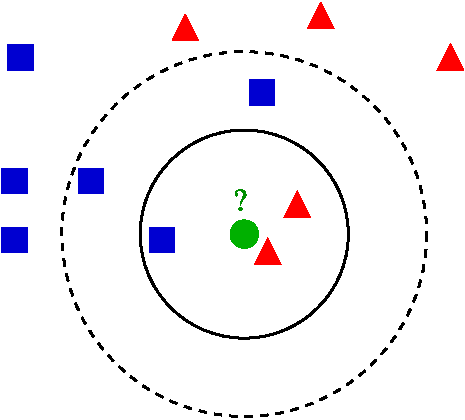
\includegraphics[width=0.4\textwidth]{images/KnnClassification}};
        \node (2) at (0.2, -1.3) {$k = 3$};
        \node (3) at (0.2, -2.6) {$k = 5$};
    \end{tikzpicture}
    \caption{Funcionamiento del algoritmo KNN \cite{knnalgorithm2010}}
    \label{fig:knn_clasification}
\end{figure}

En la Fig. \ref{fig:knn_clasification} se quiere clasificar el dato \textcolor{verdedato}{\Large$\bullet$} podemos usar múltiples valores de $k$ y con ello obtendremos diferentes resultados:
\begin{itemize}
    \item Si usamos $k = 3$ sólo nos fijaremos en los 3 datos más próximos, que serán 2 de la clase \textcolor{rojodato}{\large$\blacktriangle$} y uno de la clase \textcolor{azuldato}{$\blacksquare$}. Con esto la clase que se asignará al dato \textcolor{verdedato}{\Large$\bullet$} será \textcolor{rojodato}{\large$\blacktriangle$}.
    \item Si usamos $k = 5$ sólo nos fijaremos en los 5 datos más próximos, que serán 2 de la clase \textcolor{rojodato}{\large$\blacktriangle$} y tres de la clase \textcolor{azuldato}{$\blacksquare$}. Con esto la clase que se asignará al dato \textcolor{verdedato}{\Large$\bullet$} será \textcolor{azuldato}{$\blacksquare$}.
\end{itemize}

\subsubsection{Máquinas de vector soporte (SVM)}

Las máquinas de vector soporte son un conjunto de algoritmos de aprendizaje supervisado que se utilizan tanto para clasificación como para regresión, nos centraremos en clasificación.

Estos algoritmos toman los datos como puntos en un espacio $n-$dimensional. El objetivo es dividir estos datos mediante hiperplanos de forma que los puntos que contenidos en una región del espacio delimitada por los mismos hiperplanos sean una misma clase y que estén lo más separados posible. Esto se puede ver más fácil con un ejemplo.

En la Fig. \ref{fig:svm_separation} podemos ver como hay distintos hiperplanos ($\mathcal{H}_1, \mathcal{H}_2, \mathcal{H}_3$) que pueden dividir el espacio. 

\begin{itemize}
    \item $\mathcal{H}_1$ no divide de forma correcta todos los puntos de la entrada, puesto que hay puntos negros juntos con blancos.
    \item $\mathcal{H}_2$ sí que divide a todos los puntos en dos clases de la forma correcta, pero no están seraparas lo máximo posible de este hiperplano.
    \item $\mathcal{H}_3$ sí que cumple con las restricciones de división y distancia máxima.
\end{itemize}

\begin{figure}
    \centering
    \begin{tikzpicture}
        \node (1) {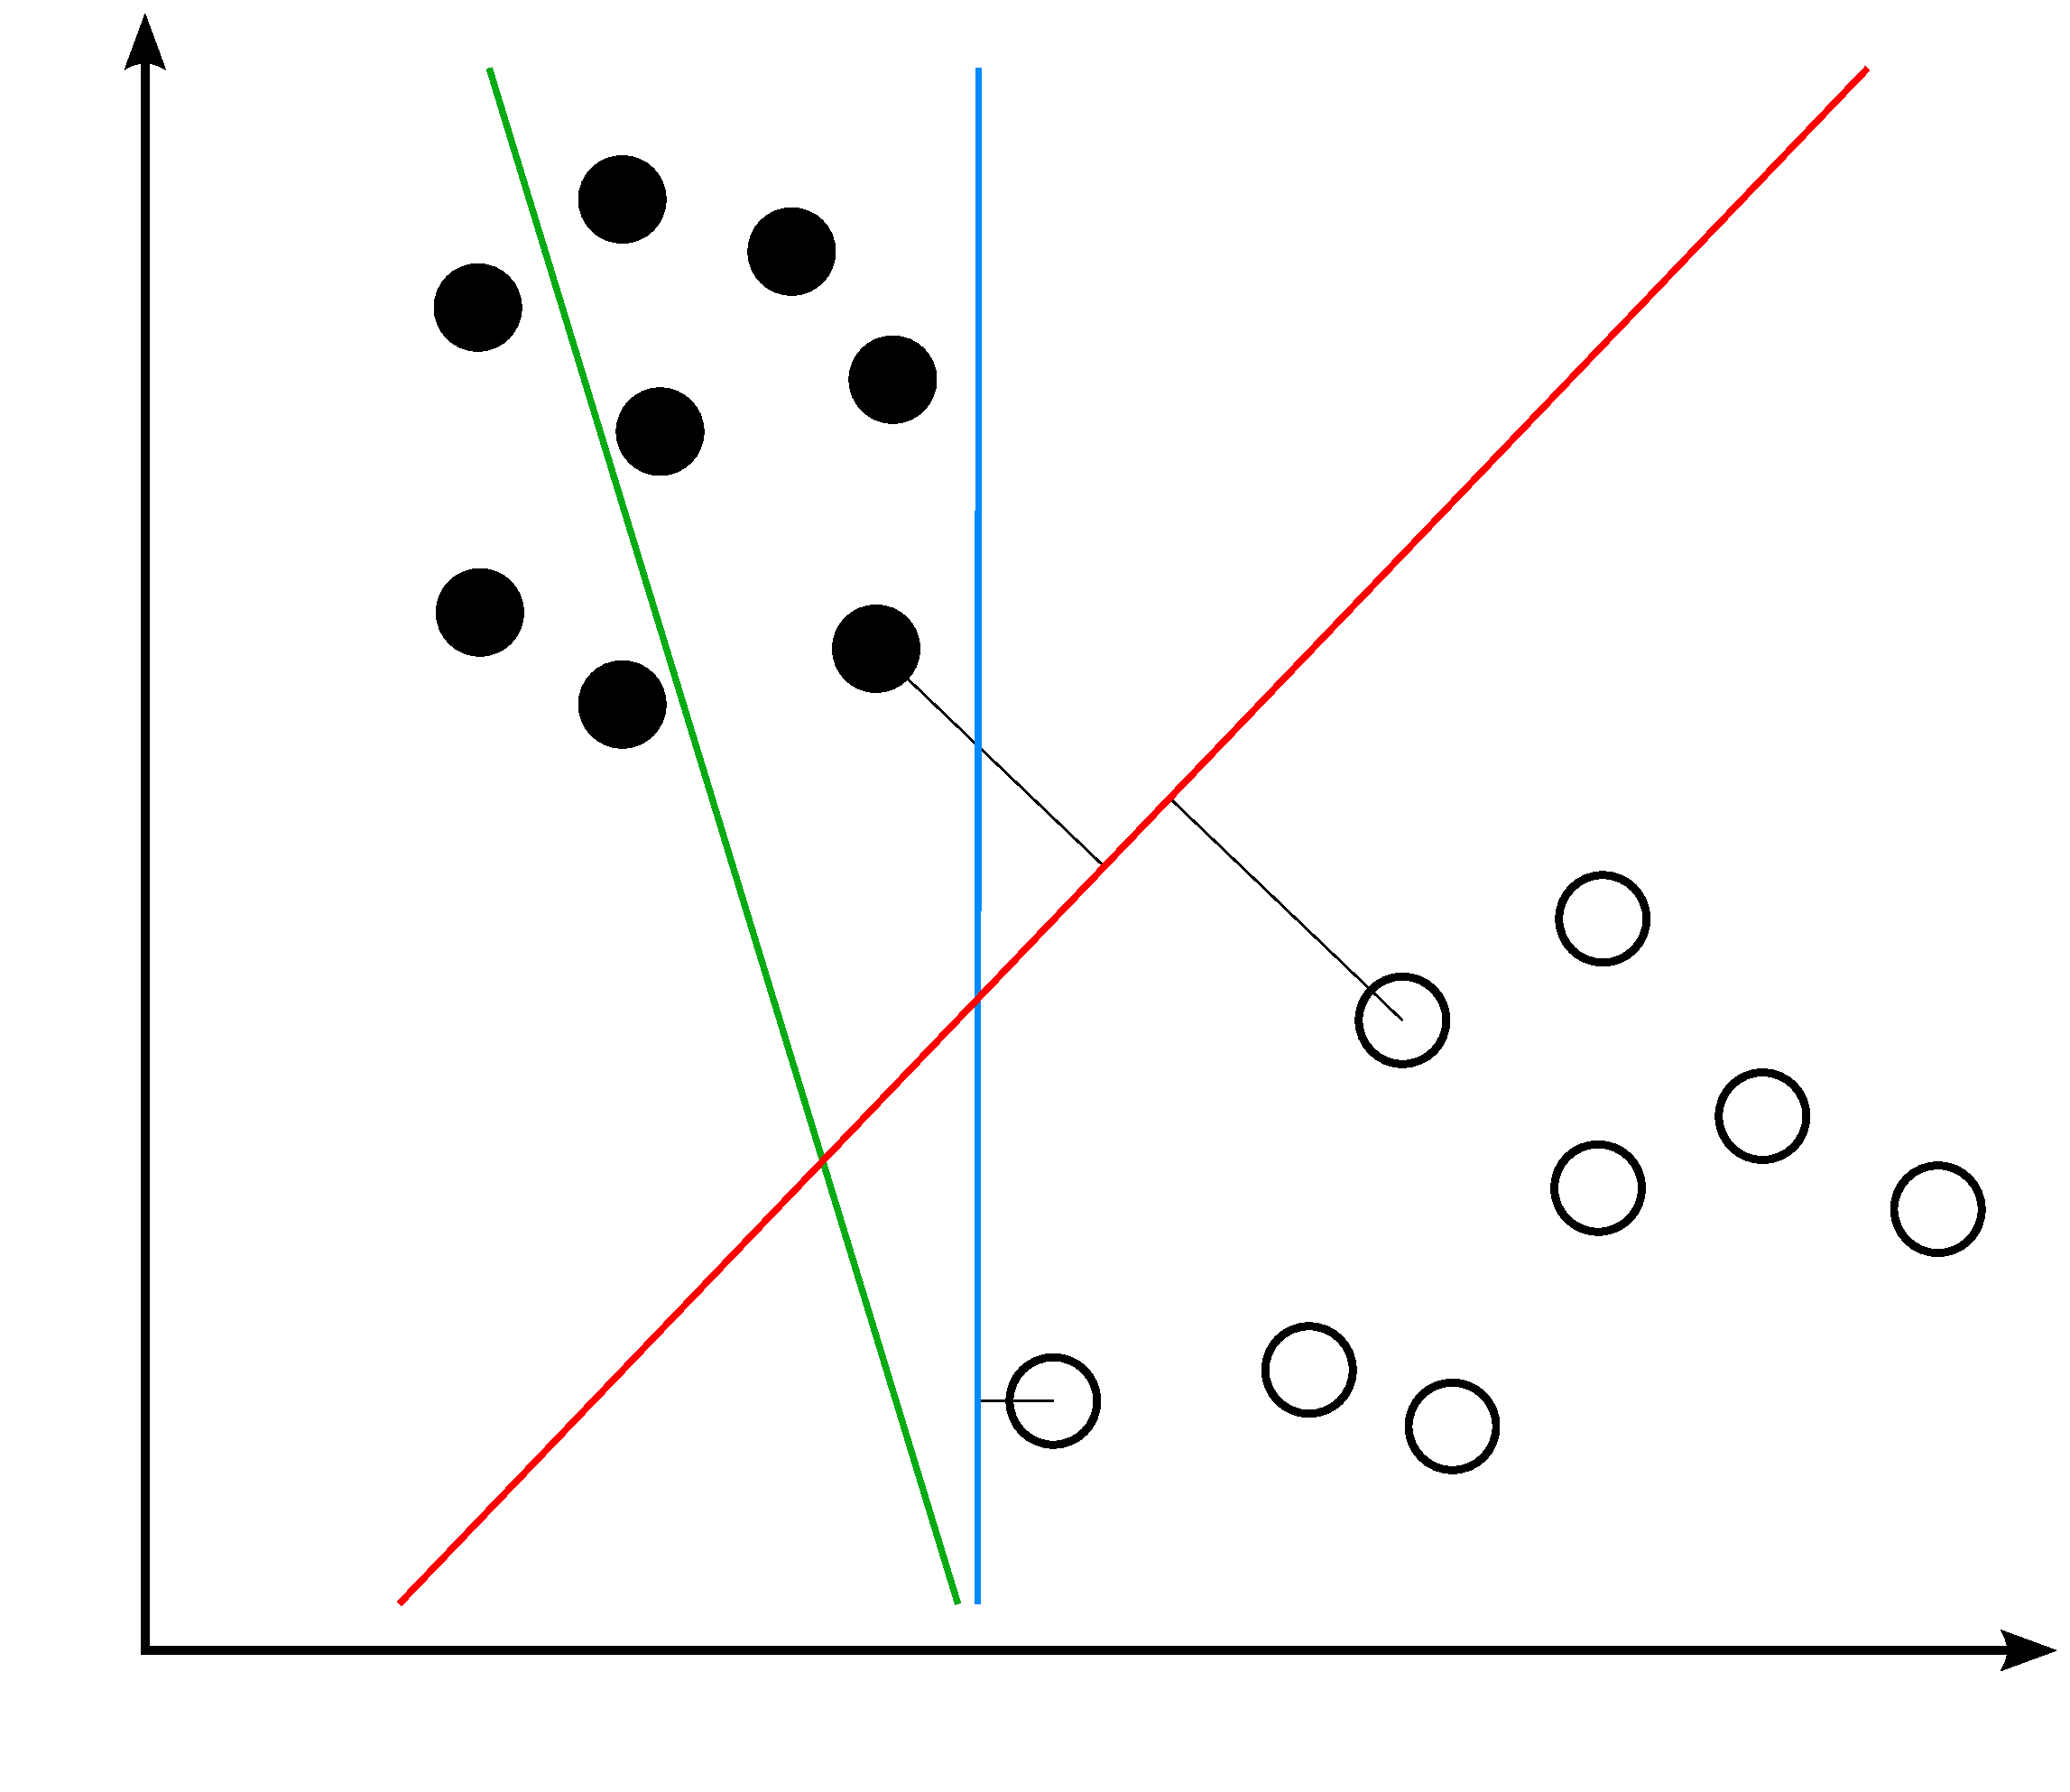
\includegraphics[width=0.4\textwidth]{images/svm_separation}};
        \node (2) at (2.7, -2.7) {$x_1$};
        \node (3) at (-3.2, 2.2) {$x_2$};
        \node (4) at (-2, 2.5) {\scriptsize $\mathcal{H}_1$};
        \node (5) at (-0.5, 2.5) {\scriptsize $\mathcal{H}_2$};
        \node (6) at (2, 2.5) {\scriptsize $\mathcal{H}_3$};
    \end{tikzpicture}
    \caption{Separación por hiperplanos SVM \cite{svmseparation2012}}
    \label{fig:svm_separation}
\end{figure}

En muchas ocasiones no se podrán dividir los conjuntos de forma correcta usando únicamente divisiones lineales del espacio, por ello, habrá que usar divisiones no lineales.